\documentclass{beamer}

\usepackage{tikz}
\usepackage{listings}
\usetikzlibrary{automata,positioning}
\usepackage{attrib}
\usepackage{color}
\usepackage{url}
\title{Verifying Type Class Laws with Equational Reasoning}
\subtitle{A description by example}
\author{Lukas Hofmaier \texttt{lukas.hofmaier@hsr.ch}}
\date{June 12, 2015 \\ Progam Analysis and Transformation Seminar FS15}

\begin{document}
\maketitle
\begin{frame}
  \frametitle{Outline}
  \tableofcontents
\end{frame}

\section{Motivation}

\begin{frame}
  \frametitle{Why I'm interested in the topic?}
 Advantages purely functional programming language?
  \begin{itemize}
  \item Higher order functions
  \item Functional programs are often shorter
  \item {\color{red} Referential transparancy makes it possible to conduct equational reasoning}
  \item It is fun
  \end{itemize}
\end{frame}

\begin{frame}
\frametitle{Referential transparency}

\end{frame}

\begin{frame}
\frametitle{Relation of type classes and equational reasonig}
\begin{figure}
  \centering
     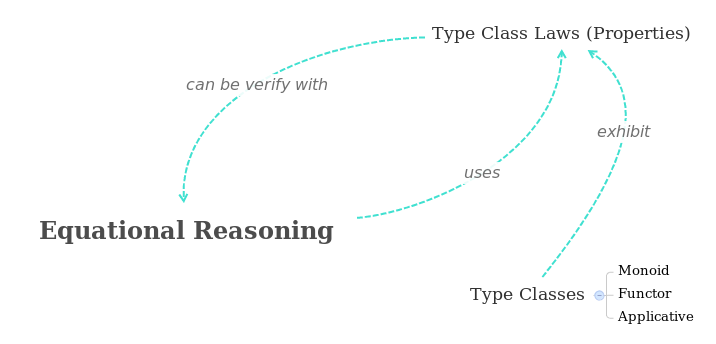
\includegraphics[scale=0.4]{mindmap}
\end{figure}
\end{frame}

\begin{frame}
 \frametitle{Why are functional programming languages great for equational reasoning?}
Referential transparancy
\end{frame}

\section{Type Classes}

\lstset{
basicstyle=\ttfamily,
columns=fullflexible,
keepspaces=true,
captionpos=b
}

\begin{frame}[fragile]
  \frametitle{Type classes support ad hoc polymorphism}

\begin{lstlisting}
showlist :: Show t => [t] -> String
showlist [] = ""
showlist (x:xs) = show x ++ showlist xs
\end{lstlisting}

\end{frame}


\begin{frame}[fragile]
  \frametitle{Monoid}
A monoid is an algebraic structure with single associatve binary operation. they are semigroups with identity
\end{frame}

\begin{frame}[fragile]
  \frametitle{An Applicative can be a monoid}
\begin{figure}
  \centering
     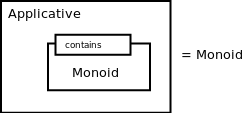
\includegraphics[width=0.7\textwidth]{monoid}
\end{figure}
\end{frame}

\section{Equational Reasoning}

\begin{frame}
  \frametitle{Comparison of testing and proving properties}
  \begin{description}
  \item[Testing] Code is compiled and executed. Can expose error. Cannot proof absence of errors. 
  \item[Proof] Properties hold under all circumstances.
  \end{description}
\end{frame}

\begin{frame}
  \frametitle{Comparison of testing and proving properties}
\begin{figure}
  \centering
     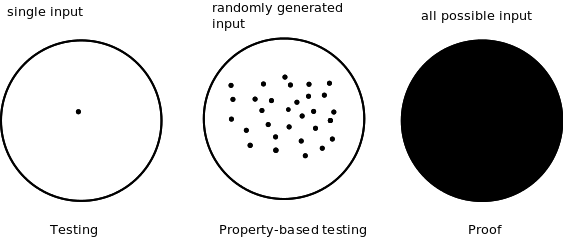
\includegraphics[width=0.7\textwidth]{testing}
\end{figure}
\end{frame}

\begin{frame}
  \frametitle{Reasoning about algebraic properties}
\begin{equation}
  \label{eq:sum}
  (x+a)(x+b) = x^2 + (a+b)x+ab
\end{equation}

\begin{equation}
  \label{eq:firstalgebra}
  (x+a)(x+b) = x^2 + ax + xb + ab \text{     (use distributivity)}
\end{equation}

\begin{equation}
x^2 + ax + xb + ab = x^2 + ax + bx + ab \text{     (use commutativity)}
\end{equation}

\begin{equation}
x^2 + ax + bx + ab = x^2 + (a + b)x + ab \text{     (use distributivity)}
\end{equation}
\end{frame}

\begin{frame}[fragile]
\frametitle{A Mickey Mouse example }
\begin{verbatim}
length [x] = 1
\end{verbatim}
\begin{lstlisting}[caption={Function definition of {\ttfamily length}},label={lst:lengthdefinition}]
length [] = 0
length (x:xs) = 1 + length xs  
\end{lstlisting}
\end{frame}

\begin{frame}[fragile]
\frametitle{Symbolic evaluation}

\begin{lstlisting}[label={lst:lengthproof}]
length [x]         -- [x] is the same as x:[]
= length (x:[])    -- apply definition
= 1 + length []    -- apply definition
= 1 + 0            --  1 + 0 = 1
1
\end{lstlisting}
\end{frame}

\begin{frame}[fragile]
\frametitle{Proof by structural induction}
 \begin{description}
 \item[Base case] Prove $p(0)$ is true.
 \item[Induction step] Prove $p(n+1)$ if $p(n)$ (induction hypothesis) is true.
 \end{description}
\end{frame}

\begin{frame}[fragile]
\frametitle{Example proof by structural induction}
The length of two concatenated lists $xs$ and $ys$, is the same as the sum of the length of $xs$ and the length of $ys$
\begin{verbatim}
length (xs ++ ys) = length xs + length ys
\end{verbatim}

\end{frame}

\begin{frame}[fragile]
\frametitle{Base case}
\begin{verbatim}
length ([] ++ ys) = length [] + length ys
\end{verbatim}
\end{frame}

\begin{frame}[fragile]
\frametitle{Induction step}
\begin{verbatim}
length ([] ++ ys) = length [] + length ys
\end{verbatim}
\end{frame}



\subsection{Applicative}

\begin{frame}
  \frametitle{For Further Reading}

  \begin{thebibliography}{Subramaniam, 2011}

\bibitem{baier08}
Graham Hutton,
Programming in Haskell,
Cambridge University Press,
2007.

\bibitem{gonzales}
Gabriel Gonzales,
Equational reasoning at scale, 
\url{http://www.haskellforall.com}.



\end{thebibliography}
\end{frame}

\end{document}
%%% Local Variables: 
%%% mode: latex
%%% TeX-master: t
%%% End: 
